\section{Reconstructed campaign decisions}
\label{sec:results}

\subsection{Qualification does not erase valid rejection reasons}

The executable reanalysis reconstructs R1 seed contrasts from the archived
loss records and checks the supplied cell and seed tables. For Paper 4,
it recomputes paired losses and candidate/null score arithmetic from 66
run-metrics records and 126 candidate score records, checking the generated
verification report. It does not rerun training, refit probes, or rescore
tensor captures. Table~\ref{tab:cohorts} lists the repetition units used
for these summaries.

\begin{table}[t]
\centering\small
\begin{tabularx}{\linewidth}{@{}lXX@{}}
\toprule
 & R1 exploration & Paper 4 pilot \\
\midrule
Candidate configurations & \RoneCells & \PfourCells \\
Repetitions per candidate & 4 training seeds & 3 paired seeds \\
Recorded scope & Frozen exploratory rules & Frozen exploratory pilot \\
Qualified breach / failed composite & \RoneQualifiedBreaches & \PfourPrivacyFailures \\
Privacy-undetermined & \RoneUndetermined & \PfourPrivacyUndetermined \\
Utility failures & \RoneUtilityFailures & \PfourUtilityFailures \\
Gain failures & \RoneGainFailures & 0 \\
Eligible candidate & None & None \\
\bottomrule
\end{tabularx}
\caption{\textbf{An empty tested feasible set has several causes.}
R1 rejection reasons overlap; Paper 4 uses its recorded composite privacy
rule. The two privacy rows are not interchangeable estimands. Counts
enumerate archived candidate configurations and carry no population
frequency interval. Sources: \artifact{R1}, \artifact{P4}.}
\label{tab:cohorts}
\end{table}

The R1 reason decomposition is decisive for interpretation. Thirteen
rejections contain a qualified breach, while the remaining six have
independent utility or gain failures. A statement that all 19 were rejected
remains correct within the frozen finite protocol. A statement that most
of those rejections were caused by unqualified instruments does not follow.
The latter would require a counterfactual repair removing the actual
rejection reasons, which these records do not provide.

The source protocols also differ in uncertainty convention. R1 uses a
two-sided 95\% seed interval; Paper 4 uses a one-sided 95\% upper limit
for utility, with $t_{0.95,2}=2.919986$ over three paired seeds. We
preserve both conventions rather than relabeling them as one common
confidence calculation. Appendix~\ref{app:checks} records the checks and
the disjoint R1 reason intersections.

Paper 4 requires a further distinction between atomic measurements and a
campaign's composite privacy label. A qualified structure probe can show a
large signal while a missing property binding leaves the recorded
all-bindings assessment undetermined. We retain both facts rather than
retroactively substituting a different aggregation policy. This preserves
the primary record and makes its scope visible. Figure~\ref{fig:campaigns}
shows the two campaigns without treating their metrics as commensurate.

\begin{figure}[t]
\centering
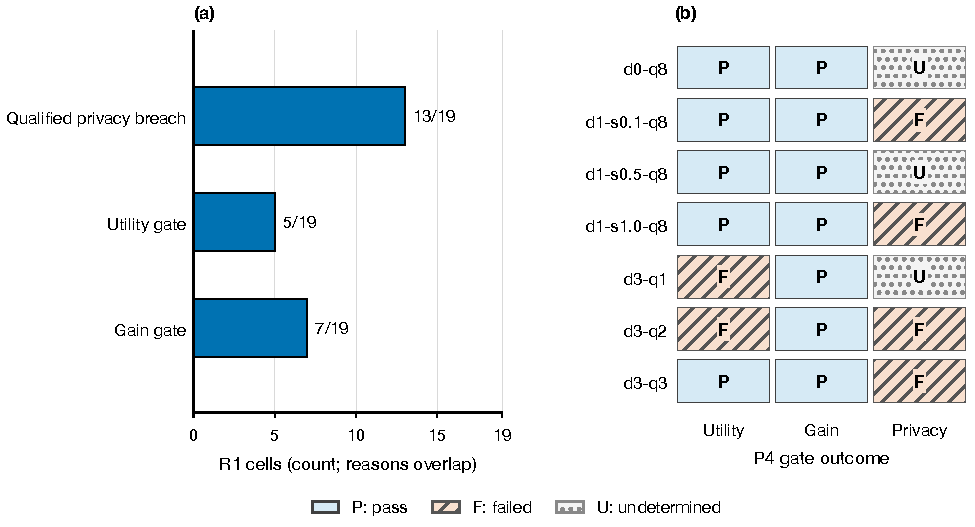
\includegraphics[width=\linewidth]{figs/campaign-gates.pdf}
\caption{\textbf{Valid negative findings coexist with incomplete coverage.}
Left: overlapping R1 rejection reasons among 19 configurations, each
evaluated with four seeds. Right: recorded gate outcomes for seven
Paper 4 cells with three paired seeds. Counts and categorical outcomes
are complete-campaign summaries, not independent population estimates;
no error bars are implied. Sources: \artifact{R1}, \artifact{P4}.}
\label{fig:campaigns}
\end{figure}

\subsection{A small margin is not a failure}

For R1, the recorded utility rule requires both the mean candidate-minus-
baseline cost to be at most $0.10$ nats and its upper 95\% Student-$t$
limit to be at most $0.12$ nats. For four seeds, the descriptive interval is
\begin{equation}
 \bar u\;\pm\;t_{0.975,3}\,\frac{s_u}{\sqrt{4}},
 \qquad t_{0.975,3}\approx3.182446.
 \label{eq:interval}
\end{equation}
These intervals are conditional on the campaign's fixed evaluation data;
they are unadjusted across configurations and are not independent corpus
replications. Figure~\ref{fig:utility} separates the two thresholds.

Span-6 has mean $0.0999705344$ and upper limit $0.1195024415$.
Its mean passes by $2.9466\times10^{-5}$ nats, and its upper limit passes
by $4.9756\times10^{-4}$ nats. The correct conclusion is not a utility
rejection caused by a rounding boundary: the saved rejection is gain
failure plus qualified privacy breach. The depth-4 point estimate is lower
than the base estimate, but neither this comparison nor the limited seed
count establishes a general depth law (\artifact{R1}).

\begin{figure}[t]
\centering
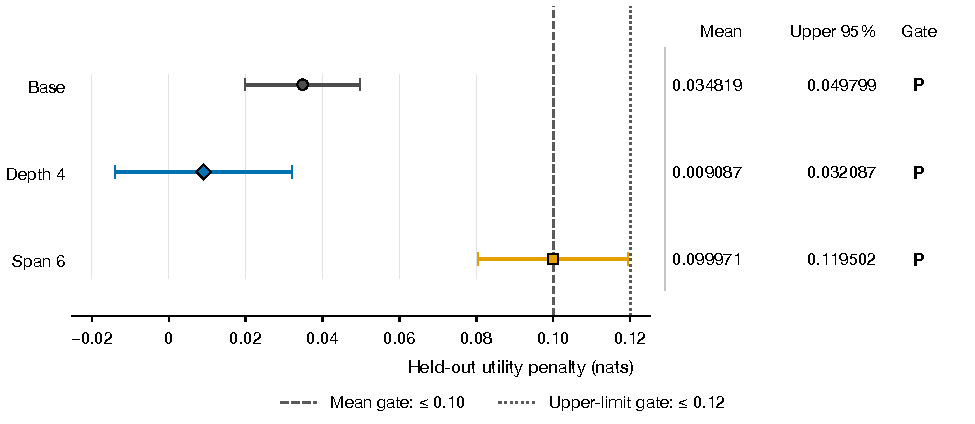
\includegraphics[width=\linewidth]{figs/r1-utility-boundary.pdf}
\caption{\textbf{Span-6 passes both recorded utility criteria.}
Means and descriptive two-sided 95\% Student-$t$ intervals across four
training seeds are conditional on fixed evaluation text. The $0.10$ mean
threshold and $0.12$ upper-limit threshold apply to different statistics;
an interval endpoint crossing the mean threshold is not itself a failure.
Source: \artifact{R1}; Eq.~\eqref{eq:interval}.}
\label{fig:utility}
\end{figure}
